Vi har køre vores naive algoritme på 20 snit i det horisontale og
vertikale plan og kommer frem til to grafer over summeringen af alle
regioner fundet i vært snit. 

Man kan se i grafen \ref{antal_regioner_vertikale_cut} for det vertikale
plan, at regionerne koncentrationen sig omkring miden af billederne.

I grafen for den horisontale plan \ref{antal_regioner_horisontale_cut}
er der tre snit som udskiller sig fra resten $91\%$, $61\%$ og $56\%$.
Hvor $91\%$ ligger højest. Fra miden af billedet og op af bliver der
fundet færre og færre regioner i snittene. Det kan skyldes at billeder med
hoisont normalt ikke har mange regioner over hoisonden, men mange under
hoisonden, eller at vores algoritme regner forkert, det første er nok det meste
sansyndlige, da vores algoritme iterere hoisontal i gemme maleriet nå vi skal
finde hoisontal regioner og vertikal nå vi finder vertikal regioner, så er
eventuel type fejl i algoritmen vil også kunne ses i den anden graf
\ref{antal_regioner_vertikale_cut}.

Hvis man samler informatioerne for de to grafer, kan man se at regionerne
samler sig fra den horisontale miden og ned af i billedet med peaker i
miden af det vertikalle plan. Det mod skrider hypotese \ref{hypo_alle_andre_snit} og \ref{hypo_midten}
og vi kan derfor forkaste dem.

\begin{figure}[h!]
	\begin{center}
		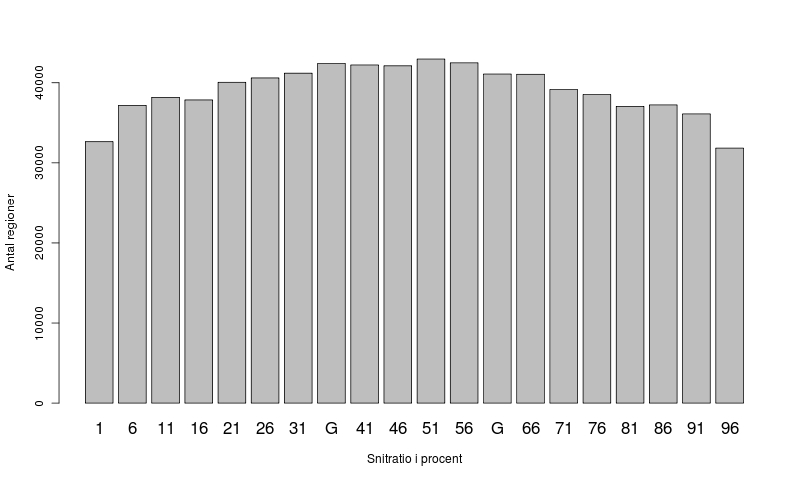
\includegraphics[width=0.9\textwidth]{afsnit/resultater/billeder/cut0cut1eatsperratio.png}
	\end{center}
	\caption{Antal regioner i hvert af de 20 vertikale snit}
	\label{antal_regioner_vertikale_cut}
\end{figure}

\begin{figure}[h!]
	\begin{center}
		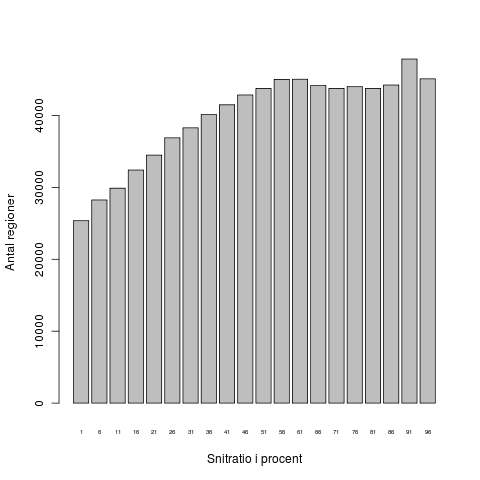
\includegraphics[width=0.9\textwidth]{afsnit/resultater/billeder/cut2cut3eatsperratio.png}
	\end{center}
	\caption{Antal regioner i hvert af de 20 horisontale snit, hvor venstre side af grafen repræsentere øverst del af malerierne}
	\label{antal_regioner_horisontale_cut}
\end{figure}

Grafe \ref{G_vs_to_trejedele} vise forskellen på antal procents vise
regioner i det gyldne snit og deres tilsvarene $\frac{2}{3}$, som man
kan se, er der ikke meget forskel på det gyldne snit og $\frac{2}{3}$ og
den største procentscise forskel ligger på $2.34\%$. Da $2.34 \% <
15\%$, må vi sige at hypotese \ref{hypo_15p} ikke, kan afviges.

I grafe \ref{G_vs_to_trejedele}, kan man også se, at selv om snittene
ligger tæt på hinanden, så har det gyldne snit en lille procents sat
flere regioner. Vi kan derfor heller ikke afvise hypotese
\ref{hypo_to_tredjedele}

\begin{figure}[h!]
	\begin{center}
		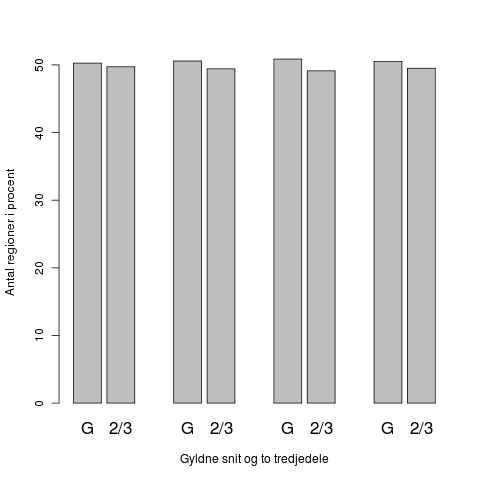
\includegraphics[width=0.6\textwidth]{afsnit/resultater/billeder/G_vs_to_tredjedele.png}
	\end{center}
	\caption{Procent vis antal regioner i de fire gyldne snit og deres tilhørene $\frac{2}{3}$ snit}
	\label{G_vs_to_trejedele}
\end{figure}

I graferne i figur \ref{naiv_year}, kan man se hvor mange regioner der
er fundet i gennemsnit per maleri i alle tidsperioder. Det ses at i
tidsperioden $(1301-1350)$ bliver der fundet ca 17 regioner per maleri,
som er klart flest. Tidsperioden (1200-1250) er den tidsperiode hvor der
bliver fundet færrest regioner, ca 7 i gennemsnit. Så der bliver fundet
mere en double så mange regioner i tidsperioder en andre. Det betyder at
hypotese \ref{hypo_tid} kan forkastes.

\begin{figure}[!h]
	\begin{center}
		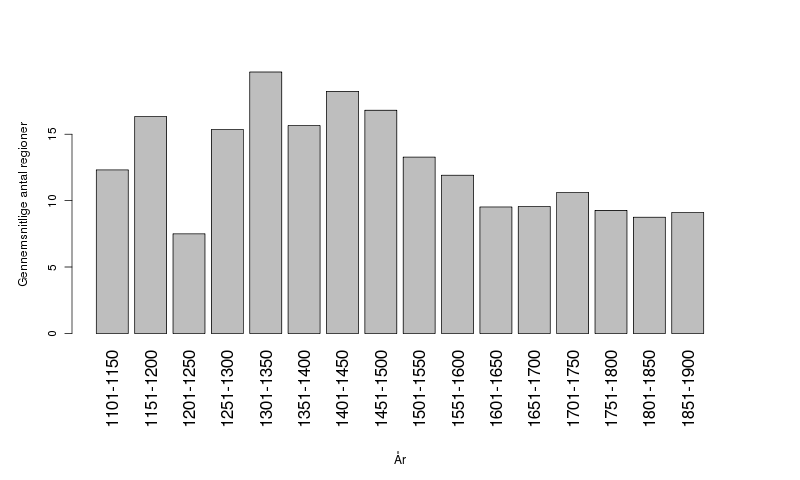
\includegraphics[angle=0,width=0.90\textwidth]{afsnit/resultater/billeder/yearcut.png}
	\end{center}
	\caption{Graf over antal regioner fundet i hver
       tidsperiode. Hver graf repræsenterer hvert deres snit. Y-aksen er
       det gemmesnitlige antal fundene regioner i snittet.}
	\label{naiv_year}
\end{figure}

I graferne i figur \ref{naiv_nation}, er samme repræsentation som
\ref{naiv_year}, bare hvor det er nationer i stegen for år. nationerne
Greek, Holland og Catala har har klart flest regioner per billedet, hvor
i mod Norge og Skotland ligger i bunden. forskellen på disse nation
ligger på ca 12, som svare til en forskel på ca $240\%$.
Da $240 \% > 10 \%$ holder hypotese \ref{hypo_nation} ikke.

\begin{figure}[!h]
	\begin{center}
		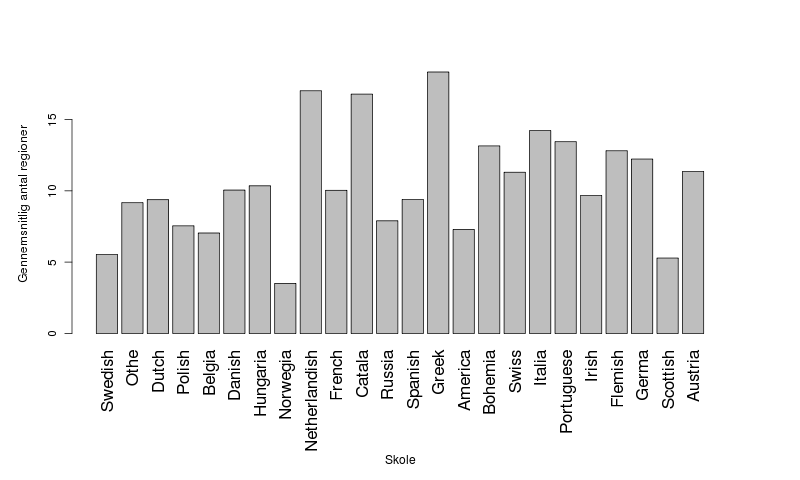
\includegraphics[angle=0,width=0.90\textwidth]{afsnit/resultater/billeder/nationcut.png}
	\end{center}
	\caption{Graf over antal fundne regioner fundet hver sin
       nationalitet. Hver graf repræsenterer hvert deres snit. Y-aksen
       er det gemmesnitlige antal fundne regioner i snittet.}
	\label{naiv_nation}
\end{figure}

